
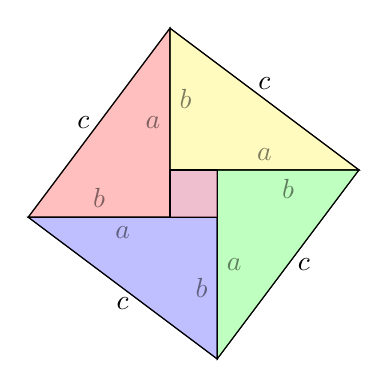
\begin{tikzpicture}[scale=.6, fil/.style={draw=black, fill opacity=.5}]
  \draw (-3,0) -- node[left] {$c$} (0,4) -- node[above] {$c$} (4,1)
    -- node[right] {$c$} (1,-3) -- node[below] {$c$} cycle
    (-3,0) -- (1,0) (0,4) -- (0,0) (4,1) -- (0,1) (1,-3) -- (1,1);
  \fill[fill=red!50, fil] (-3,0) -- (0,4) -- node[left] {$a$}
    (0,0) -- node[above] {$b$} cycle;
  \fill[fill=yellow!50, fil] (0,4) -- (4,1) -- node[above] {$a$}
    (0,1) -- node[right] {$b$} cycle;
  \fill[fill=green!50, fil] (4,1) -- (1,-3) -- node[right] {$a$}
    (1,1) -- node[below] {$b$} cycle;
  \fill[fill=blue!50, fil] (1,-3) -- (-3,0) -- node[below] {$a$}
    (1,0) -- node[left] {$b$} cycle;
  \fill[purple!50, fil] (0,0) |- (1,1) |- cycle;
\end{tikzpicture}
